\begin{figure}[H]
    \centering
    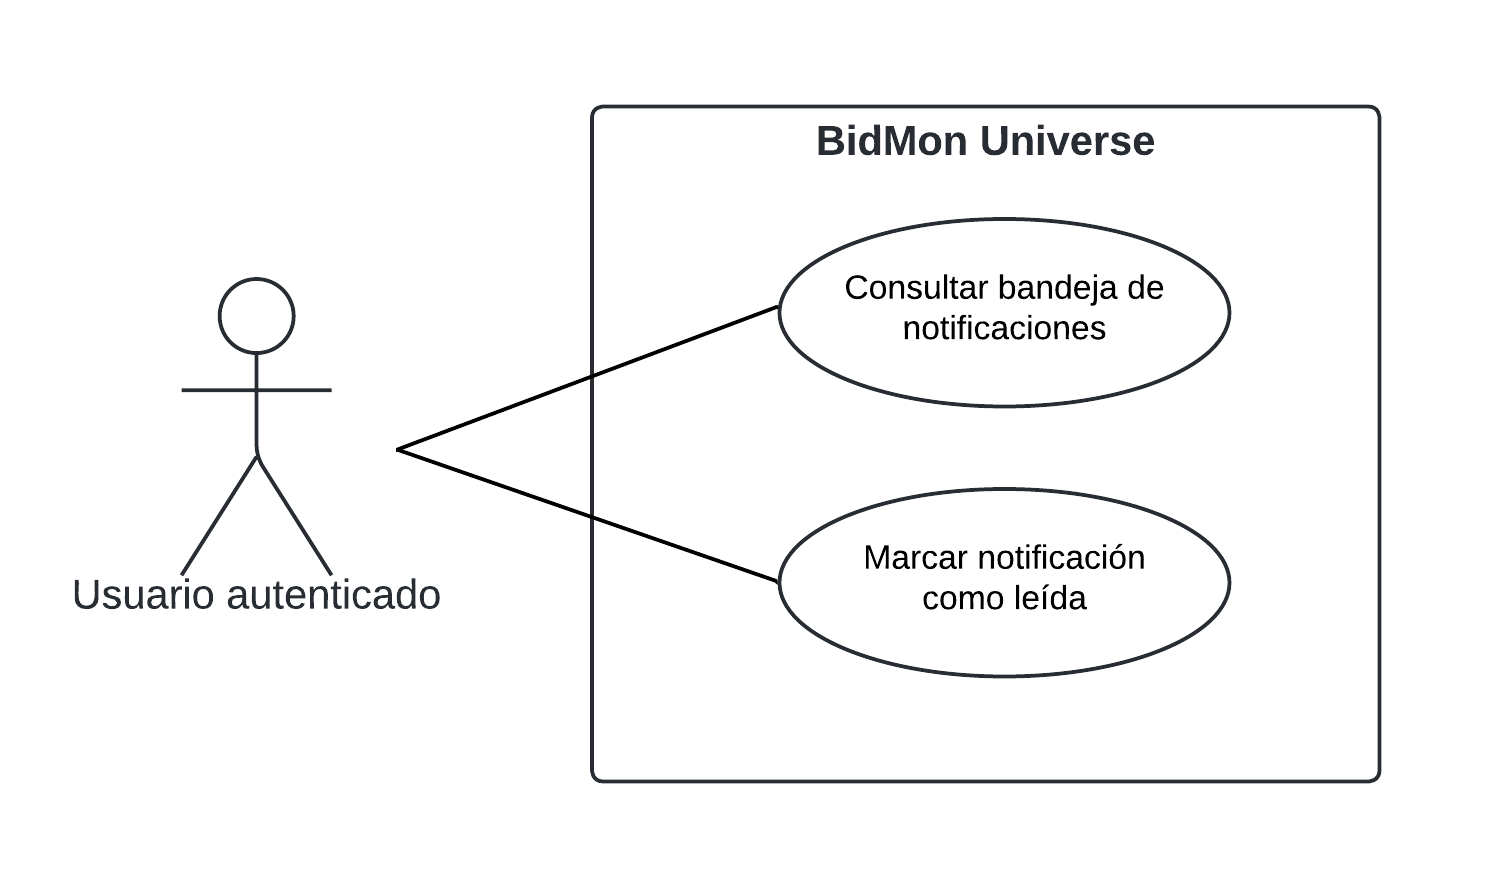
\includegraphics[width=0.5\textwidth]{figures/6-Analisis/6-Casos-uso/6_3_6_Gestion-notificaciones.png}
    \caption{Casos de uso. Gestión de notificaciones}
    \label{fig:cu_gestion-notificaciones}
\end{figure}

\subsubsection{Caso de uso. Consultar bandeja de notificaciones} \label{sec:cu_notificaciones}
\begin{longtable}{
   >{\columncolor{lightgreen!20}}p{4cm} % Primera columna con color de fondo verde claro
    >{\columncolor{white}}p{12cm}        % Segunda columna con color de fondo blanco (explícito)
    }
    \caption{Caso de uso. Consultar bandeja de notificaciones} \label{table:cu_notificaciones} \\
    \toprule
    \rowcolor{darkgreen!50} % Aplicando color de fondo verde oscuro a toda la fila
    \textbf{Caso de uso} & \centering\arraybackslash \textbf{CONSULTAR BANDEJA DE NOTIFICACIONES} \\
    \endfirsthead
    
    \multicolumn{2}{c}%
    {\tablename\ \thetable{} -- continuación de la página anterior} \\
    \toprule
    \rowcolor{darkgreen!50}
    \textbf{Caso de uso} & \centering\arraybackslash \textbf{CONSULTAR BANDEJA DE NOTIFICACIONES} \\
    \midrule
    \endhead
    
    \midrule
    \multicolumn{2}{r}{Continúa en la siguiente página...} \\ 
    \endfoot
    
    \bottomrule
    \endlastfoot
    
    \midrule
    Descripción & Un usuario autenticado puede consultar las notificaciones recibidas en el sistema. \\
    \midrule
    Actores principales & Usuario autenticado \\
    \midrule
    Actores secundarios &  \\
    \midrule
    Precondiciones & \begin{itemize}[nosep,leftmargin=*]
        \item El usuario ha iniciado sesión en el sistema.
    \end{itemize} \\
    \midrule
    Postcondiciones &  \\
    \midrule
    Disparadores & El usuario accede a la sección de notificaciones. \\
    \midrule
    Escenario principal & \begin{enumerate}[nosep,leftmargin=*]
        \item El sistema muestra el listado de notificaciones recibidas por el usuario.
    \end{enumerate} \\
    \midrule
    Escenarios alternativos & 
    \begin{itemize}[nosep,leftmargin=*]
        \item \textbf{Escenario alternativo 1. No hay notificaciones.}
        \begin{enumerate}[nosep,leftmargin=*]
            \item El sistema muestra un mensaje indicando que no hay notificaciones.
        \end{enumerate}
    \end{itemize} \\
    \midrule
    Situaciones de error & 
    \begin{itemize}[nosep,leftmargin=*]
        \item \textbf{Error de conexión a la base de datos.}
        \begin{enumerate}[nosep,leftmargin=*]
            \item El sistema muestra un mensaje de error.
        \end{enumerate}
    \end{itemize} \\
\end{longtable}

\subsubsection{Caso de uso. Marcar notificación como leída} \label{sec:cu_marcar-leida}
\begin{longtable}{
   >{\columncolor{lightgreen!20}}p{4cm} % Primera columna con color de fondo verde claro
    >{\columncolor{white}}p{12cm}        % Segunda columna con color de fondo blanco (explícito)
    }
    \caption{Caso de uso. Marcar notificación como leída} \label{table:cu_marcar-leida} \\
    \toprule
    \rowcolor{darkgreen!50} % Aplicando color de fondo verde oscuro a toda la fila
    \textbf{Caso de uso} & \centering\arraybackslash \textbf{MARCAR NOTIFICACIÓN COMO LEÍDA} \\
    \endfirsthead
    
    \multicolumn{2}{c}%
    {\tablename\ \thetable{} -- continuación de la página anterior} \\
    \toprule
    \rowcolor{darkgreen!50}
    \textbf{Caso de uso} & \centering\arraybackslash \textbf{MARCAR NOTIFICACIÓN COMO LEÍDA} \\
    \midrule
    \endhead
    
    \midrule
    \multicolumn{2}{r}{Continúa en la siguiente página...} \\ 
    \endfoot
    
    \bottomrule
    \endlastfoot
    
    \midrule
    Descripción & Un usuario autenticado puede marcar una notificación como leída. \\
    \midrule
    Actores principales & Usuario autenticado \\
    \midrule
    Actores secundarios &  \\
    \midrule
    Precondiciones & \begin{itemize}[nosep,leftmargin=*]
        \item El usuario ha iniciado sesión en el sistema.
    \end{itemize} \\
    \midrule
    Postcondiciones &  El sistema marca la notificación como leída en la base de datos y registra la fecha y hora de lectura. \\
    \midrule
    Disparadores & El usuario accede a la sección de notificaciones y selecciona una notificación. \\
    \midrule
    Escenario principal & \begin{enumerate}[nosep,leftmargin=*]
        \item El sistema muestra el listado de notificaciones recibidas por el usuario.
        \item El usuario selecciona una notificación.
        \item El sistema marca la notificación como leída.
    \end{enumerate} \\
    \midrule
    Escenarios alternativos & 
    \begin{itemize}[nosep,leftmargin=*]
        \item \textbf{Escenario alternativo 1. Marcar todas las notificaciones como leídas.}
        \begin{enumerate}[nosep,leftmargin=*]
            \item El sistema muestra la opción de marcar todas las notificaciones como leídas.
            \item El usuario selecciona la opción de marcar todas las notificaciones como leídas.
            \item El sistema marca todas las notificaciones como leídas.
        \end{enumerate}
    \end{itemize} \\
    \midrule
    Situaciones de error & 
    \begin{itemize}[nosep,leftmargin=*]
        \item \textbf{Error de conexión a la base de datos.}
        \begin{enumerate}[nosep,leftmargin=*]
            \item El sistema muestra un mensaje de error.
        \end{enumerate}
    \end{itemize} \\
\end{longtable}

